\documentclass{standalone}

\usepackage{tikz}
\usepackage{bm}
\usepackage{amsmath}
\usetikzlibrary{calc, tikzmark, shapes, shapes.arrows, arrows, positioning}
\newcommand{\mat}[1]{\boldsymbol{\rm{#1}}}
\newcommand{\T}{\mat{T}}
\renewcommand{\vec}[1]{\boldsymbol{#1}}
\newcommand{\x}{\boldsymbol{\mathrm{x}}}

\begin{document}
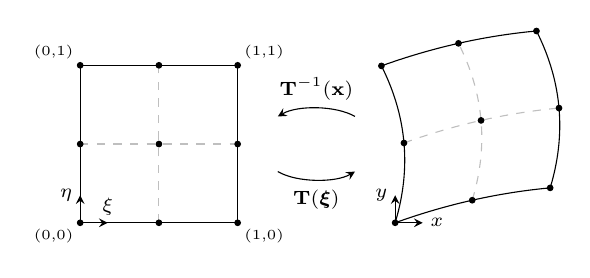
\begin{tikzpicture}
	\scriptsize
	\draw (0,0) grid[step=2] (2,2); 
	\foreach \x in {0,1,2} {
		\foreach \y in {0,1,2} {
			\filldraw (\x,\y) circle[radius=1pt]; 
		}
	}
	\draw[dashed, opacity=.25] (1,0) -- (1,2); 
	\draw[dashed, opacity=.25] (0,1) -- (2,1);
	\draw[->, >=stealth] (0,0) -- (.35,0) node[above] {$\xi$}; 
	\draw[->, >=stealth] (0,0) -- (0,.35) node[left] {$\eta$}; 
	{
		\tiny
		\node[below left] at (0,0) {(0,0)}; 
		\node[below right] at (2,0) {(1,0)}; 
		\node[above left] at (0,2) {(0,1)}; 
		\node[above right] at (2,2) {(1,1)}; 
	}

	\begin{scope}[xshift=3cm, yshift=1cm]
		\draw[->, >=stealth, shorten >= 3mm, shorten <= 3mm] (-.75,-.2) to [bend right=30] (.75,-.2); 
		\node at (0,-.7) {$\T(\vec{\xi})$}; 
		\draw[->, >=stealth, shorten >= 3mm, shorten <= 3mm] (.75,.2) to [bend right=30] (-.75,.2); 
		\node at (0,.7) {$\T^{-1}(\x)$}; 
	\end{scope}

	\begin{scope}[scale=2, yshift=0cm, xshift=2cm]
	\draw plot[samples=100, domain=0:1, variable=\t]({.311322*\t-.398478*\t^2}, {1.03106*\t-.0348623*\t^2}); 
	\draw plot[samples=100, domain=0:1, variable=\t]({0.984429 + 0.311322*\t - 0.398478*\t^2}, {0.221642 + 1.03106*\t - 0.0348623*\t^2}); 
	\draw plot[samples=100, domain=0:1, variable=\t]({0.973098*\t + 0.0113302*\t^2}, {0.351147*\t - 0.129505*\t^2}); 
	\draw plot[samples=100, domain=0:1, variable=\t]({-0.0871557 + 0.973098*\t + 0.0113302*\t^2}, {0.996195 + 0.351147*\t - 0.129505*\t^2}); 
	\draw[dashed, opacity=.25] plot[samples=100, domain=0:1, variable=\eta]({0.489382 + 0.311322*\eta - 0.398478*\eta^2}, {0.143197 + 1.03106*\eta - 0.0348623*\eta^2}); 
	\draw[dashed, opacity=.25] plot[samples=100, domain=0:1, variable=\xi]({0.0560416 + 0.973098*\xi + 0.0113302*\xi^2}, {0.506813 + 0.351147*\xi - 0.129505*\xi^2}); 
	\filldraw (0.00000000,0.00000000)  circle[radius=.5pt]; 
	\filldraw (0.48938177,0.14319734)  circle[radius=.5pt]; 
	\filldraw (0.98442867,0.22164203)  circle[radius=.5pt]; 
	\filldraw (0.05604160,0.50681292)  circle[radius=.5pt]; 
	\filldraw (0.54542337,0.65001026)  circle[radius=.5pt]; 
	\filldraw (1.04047027,0.72845495)  circle[radius=.5pt]; 
	\filldraw (-0.08715574,0.99619470) circle[radius=.5pt]; 
	\filldraw (0.40222603,1.13939204)  circle[radius=.5pt]; 
	\filldraw (0.89727293,1.21783673)  circle[radius=.5pt]; 
	\draw[->, >=stealth] (0,0) -- (.35/2,0) node[right] {$x$}; 
	\draw[->, >=stealth] (0,0) -- (0,.35/2) node[left] {$y$}; 
	\end{scope}
\end{tikzpicture}
\end{document}